\documentclass[a4paper]{article}
\usepackage{html}
\usepackage{graphicx}
\usepackage{ifpdf}
\newcommand{\oofem}{\htmladdnormallink{OOFEM}{http://www.oofem.org}\ }
\newcommand{\bp}{\htmladdnormallink{Bo\v{r}ek Patz\'{a}k}{http://mech.fsv.cvut.cz/~bp/bp.html}}

\renewcommand{\topfraction}{0.99}	% 99% of page top can be a float
\renewcommand{\bottomfraction}{0.99}	% 99% of page bottom can be a float
\renewcommand{\textfraction}{0.01}	% only 1% of page must to be the text
\renewcommand{\floatpagefraction}{0.99} % 99% of whole page can be a float
\setcounter{totalnumber}{5} %maximum floating objects on one page


\newcommand{\class}[1]{{\bf #1}}
\newcommand{\service}[1]{{\em #1}}
\begin{document}
%begin{latexonly}
\title{Object Oriented\\ Finite Element Modeling\footnote{When
referencing this paper, please cite the following: Patz\'{a}k, B.:
{\em Object oriented finite element modeling}, ACTA POLYTECHNICA, 39(2/1999):99-113, 1999. ISSN 1210-2709}}
\author{\bp \\ \\
Czech Technical University\\
Faculty of Civil Engineering\\
Department of Structural Mechanics\\
Th\'akurova 7, 166 29 Prague, Czech Republic
}
\maketitle
%end{latexonly}
\begin{htmlonly}
\begin{center}
{\Large Object Oriented\\ Finite Element Modeling\footnote{When
referencing this paper, please cite the following: Patz\'{a}k, B.:
{\em Object oriented finite element modeling}, ACTA POLYTECHNICA, 39(2/1999):99-113, 1999. ISSN 1210-2709}}s
{\bp \\ 
Czech Technical University\\
Faculty of Civil Engineering\\
Department of Structural Mechanics\\
Th\'akurova 7, 166 29 Prague, Czech Republic\\ \\
}
\end{htmlonly}

\noindent{{\bf Key words:} Finite Element Modeling, Object Oriented Analysis}

\abstract{
This paper presents a general structure of an object oriented finite element code. 
The aim of the described object oriented environment is not only to be
an efficient and robust tool for FEM computations, but also to provide
a modular and extensible tool for new developments.	
The program structure has been designed to meet all natural
requirements for modularity, extensibility, and robustness. Special
attention is put on the description of the representations and
interfaces of the material model and the analysis module.
For reader convenience, a short introduction to Object Oriented
Analysis is given. The program structure design presented has been
successfully implemented. }


\section{Introduction}

During the last decades engineering community has been facing a rapid
development in many related fields. Also the recent progress in
computer technology allows the practical use of many advanced, complex, and large FE models. 
%%Due to these facts, five years ago we were looking for suitable environment for our FEM computations. We wanted to find out code which is easily extensible toward future demands, easily maintainable, but still efficient and portable across many platforms. 
Due to these facts, the necessity for a suitable FEM computation
environment is evident. An analyst or researcher naturally wants to
work with code which is easily extensible towards future demands, easily maintainable, but still efficient and portable across many platforms. 

Generally, there are two main groups of  existing programs. 
The first group consists of commercial products available on the market. These codes
are offering wide functionality including many different analysis procedures,
wide element libraries and are often provided with pre- and post-
processing tools. Despite these facts, these packages are designated
mainly to end users in design offices, providing excellent
tools for standard types of analyses. The main disadvantage is their
very limited or even impossible extensibility. Usually a set of user
defined subroutines is provided. By using these subroutines, the addition
of a new element type or the introduction of a new constitutive
laws is theoretically possible. Nevertheless, the extension to a new analysis
type or the extension to a principally new material model with required
history variables can be hardly possible. Therefore, these programs
are oriented towards practical computations, rather than to the
research engineering community.  
The second group of available programs is represented by programs
distributed with source codes. In-house programs as well as many free-
and share-ware programs were analysed and tested to determine whether they fulfilled
required needs. 
%%These programs were not or very poorly modular. 
They usually proved to be entirely inmodular or very poorly
modular. Extensibility, primarily of interest to a researcher, is enabled
due to existence of source code, but it is extremely time consuming
and error prone due to unclear data structure or bad program
design. This is further complicated by missing or insufficient
documentation. 
%Also, as a consequence of poor modularity, team work is hardly
%possible.
Also, as a consequence of poor modularity, the distributed software
development within a team is hardly possible.


%%(slide project goals)
Due to the aforementioned facts, a new general FEM kernel has been designed and developed 
with several modules being built on its top.
The kernel provides the basic common services and data
structures. 
%Modules are implementing module dependent parts. 
Particular modules are designed to implement analysis specific parts by extending
and specializing the basic kernel structure represented by its
services and data structures. The module must provide problem
formulation, numerical algorithms, finite elements and other
necessary components for a specific analysis.
At the very beginning, the following project goals were formulated:
\begin{itemize}
\item
The most important requirement from the research community point of view, was to
achieve an open nature of the kernel library - extensibility in a broad sense. The
kernel has to be extensible in
any ``direction''. Thus the possibility of adding new element types, new
material models with any type and number of internal history variables,
new boundary conditions or new analysis modules, must be a matter of
course. 
\item
The program structure must comply with a modular design. This
is a very important feature to support team work. 
%%Also of great importance is modular design of program structure. This
%%is also very important for team work support. 
\item
The code must be easily modifiable and maintainable. The important and
natural requirement for a program is its portability over available
and future platforms.
\item
Although extensibility and easy maintenance were of primary concern,
the last but not least item --- the efficiency is also a very
important property, mainly from the viewpoint of the end user. We expected
to obtain computational performance similar to programs
written in Fortran or C. The minor decrease in speed is not 
important, if we realize the progress in computer hardware technology.
\end{itemize}


%%(slide methods)
\section{Object Oriented Analysis}
A short outline of Object Oriented Analysis (OOA) will be given here, to
help the reader to understand
the basic principles of the subject. The basic terms and
principles necessary for understanding of program structure, used
later in this paper, will be mentioned and explained. 
Object Oriented Analysis  is based on the uniform application of 
principles for managing complexity (see Ref.~\cite{CoadYourdon}).
\begin{itemize}
\item[-]
Abstraction (Procedural and data abstraction): The principle of ignoring
those aspects of a subject that are not relevant to the current purpose
in order to concentrate more on those that are relevant.
\item[-]
Procedural abstraction: The principle that any operation that achieves
a well defined effect can be treated by its users as a single entity,
despite the fact that the operation may be actually achieved by some
sequence of low level operations. Procedural abstraction is widely
supported by existing programming languages; procedures and functions
are examples of procedural abstraction.
\item[-]
Data abstraction: The principle of defining a new data type in terms of
the operations that apply to an object of that type, with the constraint
that the values of such an object can be modified and observed only by
the use of the operations. When applying data abstraction, an analyst
must define attributes and services that exclusively
manipulate these attributes. The only way, to get an attribute is via
these services.
\item[-]
Inheritance: The mechanism for expressing similarity between data types,
making common attributes and services explicit within a class
hierarchy. Inheritance allows an analyst to define common attributes
and services only once, as well as to specialize and extend those
attributes and services into specific derived classes. It expresses
generalization specialization between data types.
\item[-]
Association: Expresses the relationship, the state of being associated. 
\item[-]
Communication with messages: Models the processing dependency. It
represents the need for services necessary to fulfill object responsibility.
\end{itemize}

%%In an overall approach, OOA consist of five major activities
%%\begin{itemize}
%%\item
%%Finding class and object.
%%\item
%%Identifying structures.
%%\item
%%Identifying subjects.
%%\item
%%Defining attributes.
%%\item
%%Defining services.
%%\end{itemize}
In an overall approach, OOA consists of five major activities: finding classes and objects, identifying structures, identifying subjects, defining attributes, and defining services.
In order to present the general structure of a developed program, 
a graphical form will be used. Particularly, the Coad-Yourdon methodology
will be used (see Ref.~\cite{CoadYourdon}). It introduces the following basic elements and mutual
relations between them (see Fig.~1.):

%\fig[h]{0mm\centerline{\epsfbox{coyoSm.eps}}}           %obr.1
%{General Structure}

\begin{itemize}
\item
An {\em Object} is an abstraction of something in a problem domain, reflecting
the capabilities of a system to keep information about it, interact
with it, or both. It is also an encapsulation of attribute values and
their exclusive services. A Synonym for object is an instance.
\item
{\em Class}: A description of one or more objects with a uniform set of
attributes and services, including a description of how to create a new
object in a class.
\item
{\em Class \& object}: A term meaning class and the objects in that class. 
\item
{\em Attributes} describe the values (state) of the object, to be
exclusively manipulated by the services of that object. The attributes
and exclusive services on those attributes are assumed as an intrinsic
whole. If another part of a system (another object) needs to access or
otherwise manipulate the values in an object, it must do so by
specifying a message connection corresponding to service defined for
that object.
\item
{\em Services}: The central issue in defining services is to define required
behavior and necessary communication.
\item
Generalization specialization structure may be viewed as a layout for
distinguishing between classes.  Less formally, a {\em Genspec} structure
can be thought to be an expression for ``is a'' or ``is a kind of''
relation. Within a Genspec structure inheritance applies. An example
is the generalization class \class{Vehicle} and specialization class \class{Truck
vehicle}. Genspec structure is represented by generalization class
and by specialization class with a line drawn between them. A
semi-circle mark distinguishes classes as forming Genspec
structure. The notation is directional --- it uses a line drawn outward
from semi-circle midpoint to point to the generalization (see Fig.~1.). 
\item
{\em Whole part structure} groups together class\&objects based upon
whole-part meaning. This structure is represented by a whole object and
by a part object, with a line drawn between them. A triangle mark
distinguishes the object as forming the whole part structure. The notation is
again directional. Each end of whole part structure line is marked
with amount or range, indicating the number of parts that the whole may
have and vice versa, at any given moment in time. The alternative
modeling is to use an instance connection. It is weaker in meaning, but
it still captures the mapping (see Fig.~1.). 
\item
Attributes depict the object state. Instance connections add to this
information, which required mappings are needed by an object to fulfill
its responsibilities. Instance connections model association. A
connection is represented by a line drawn between objects. Each object
can again have an amount or range marks on each of its instance
connections, reflecting constraints with other objects.
\item
A message connection is a mapping of one object to another (or
occasionally to a class, to create a new object), in which a sender
sends a message to a receiver, to get some processing done. The needed
processing is named in the sender's service specification, and is defined
in the receiver's service specification. The benefit of such a discipline
is that it creates a very narrow interface between the strong
encapsulation and exclusive services on those data. In effect, a
message connection combines event-response and data flow perspectives.
Each message represents values sent within the context of
particular service need, and a response received as result.
\end{itemize}


\section{General Structure}
%Let us move to the next part of presentation, to the description of
%structure of  OO FEM program.

General structure is shown in Fig.~2.
First focus attention on the class \& object \class{Domain}. Generally
speaking, it contains the problem description, or if the program runs in
parallel, then it contains the description of the domain associated
with a particular processor or thread of execution. \class{Domain} 
contains and manages lists of degree of freedom (DOF) managers, elements, boundary
conditions, cross sections, and materials - these describe the geometry
of problem, its constitutive properties, and applied boundary
conditions. Services for accessing each of these objects are
provided. \class{Domain} class \& object contains also several \class{Engineering
model}s. These objects represent the type of analysis, which may be
invoked. 
\class{Domain} class \& object provides services for reading input
files, and instantiating corresponding components accordingly. \class{Domain},
after reading problem description and performing necessary consistency
checks, starts computation by sending appropriate message to
\class{Engng model}.



%\fig[t]{0mm\label{genstructfig}\centerline{\epsfbox{generalSm.eps}}}           %obr.1
%{General Structure}

Engng model and Numerical method interfaces, shown schematically in
top-left frame, will be explained in section~\ref{engngNummetsection}
The classes \& objects in the left-bottom frame represent the element,
material model, and cross section abstractions. Because of their
principal importance, a special 
section~\ref{materialEleemntFrame} will be devoted to a detailed
explanation of this frame. 

\class{DOF} is an abstraction for a single degree of freedom (DOF). It maintains
its physical meaning and associated equation number. \class{DOF} is
the attribute of
one \class{DofManager}. The \class{DofManager} manages the collection
of DOFs. A typical
derived class is class \class{Node}, representing a node in a finite element mesh.
\class{Boundary condition} and \class{Initial condition} are abstractions of boundary and
initial conditions. They are attributes of \class{Domain} and are associated
with one or more \class{DOF}s. The abstract class \class{Load}, derived from base \class{Boundary
condition} class, is an abstraction for load. It is an attribute of \class{Domain}
and can be associated with several dof managers or elements, according to
the type. The class declares the basic services provided by
all derived classes. Derived classes declare specific load type dependent
services and implement all necessary services.



\section {Engineering model --- Numerical Method Interface}
\label{engngNummetsection}

\class{Engng model} is an abstraction for the type of analysis, that will be
done. Base class offers basic general services for assembling
characteristic components and services for starting the solution step and
its termination. Derived classes ``know'' the form of governing
equation and the physical meaning of  particular components. 
They are responsible for forming the governing equation for each solution
step, which may represent either a time step, a load increment, or a load
case, usually by summing contributions from particular elements and nodes.
In order
to solve the governing equation, a suitable instance of \class{Numerical Method}
class is created. \class{Engng model} may use different numerical methods,
depending, for example, on problem size or previous convergence. \class{Engng
model} first maps its components of the governing equation (for example
stiffness matrix, load vector) to corresponding numerical components
(LHS, RHS), and then sends a message to the appropriate numerical method to solve the
problem (see Fig.~4). 
\class{Engng model} must also provide services for updating its
components, if this is necessary. These are used, when the \class{Numerical
Method} instance needs to update  some components during solution (for
example in the Newton Raphson algorithm for the solution of non-linear
equations, stiffness has to be updated after each
iteration). Similarly,  
a high-level numerical method may use the services of another
low-level numerical method (solver for non-linear system  of equations
uses another linear solver for linearized problem). \class{Numerical method}
instance may also represent an interface to some procedure in C or
Fortran (see Fig.~4.). 

%In this picture, you can see the interface of numerical method
%class. 
%Interface of Numerical method is schematically shown on fig. xx.
%Here, engng model represented by class eigen value dynamic,
%which as name indicates, represent dynamic eigen value problem. After
%it assembles its global stiffness and mass matrices, it creates
%suitable instance of  numerical method to solve the problem. Subspace
%iteration method has been selected here.

%\fig[t]{0mm\label{engngNummet1fig}\centerline{\epsfbox{struct2Sm.eps}}}           %obr.2
%{Engng model - Numerial method Interface}

One important aspect, which should be mentioned here, is that all
numerical methods solving the same problem use the same names for numerical
components. This is important, because the
situation, where different numerical methods use different message
names and parameter ordering for the same service is avoided. This is
necessary, otherwise any future introduction of numerical method
could require some necessary code changes. However, by using the
proposed compulsory mapping of each component separately to
compulsory (and common) component names, it is possible to create a new
instance of \class{Numerical method}, and leaving the whole engineering model code
including mapping unchanged. 

This concept is further enhanced by introduction of base abstract
class for all sparse matrices. This class only declares the basic
required services provided by all sparse matrices (like multiplication
by a vector, possible factorization, etc). The implementation is left on
derived classes.  Numerical methods are then implemented only
using basic services declared by \class{Sparse Matrix} class. Thus, numerical
methods class instances will work with any sparse matrix class, even
those added in the future, without changing any code, because all derived
classes of \class{Sparse Matrix} class implement the same interface.

\subsection {Program \& Data Flow}
%%(slide frame 3 - program flow engng model - numerical method)
The program flow in the engineering model --- numerical method frame is 
explained in Fig.~3. After \class{Domain} reads the input file with
the problem description,
it starts computation by invoking \service{SolveYourself} service of \class{Engng
model} class. In this example a non-linear static problem
analysis is performed. The corresponding \class{Engng model} class solves the whole problem
as a series of load increments. Therefore, for each step of computation,
a \service{SolveYourselfAt} service is invoked. For the first step, the reference
load vector is formed from element and nodal contributions, so these
components are accessed from corresponding domain using its
services. Then, for each solution step,  the stiffness matrix is formed
and particular components of the governing equation are mapped to
the numerical method components. Here, an \class{CALM} instance of \class{Numerical
Method} class is being used. For solution of a linearized problem, the
\class{CALM} uses another instance of \class{Numerical method} class - here named
\class{Linear solver}. After components are mapped and a solution is obtained,
the \class{CALM} checks convergence. It asks \class{Engng model} to compute
(update) the vector of real nodal forces according to the solution reached,
and checks convergence. If convergence is reached, the program control
returns to \class{Engng model} and the solution step is then terminated (stress
updates and necessary printing) and the solution continues with next
step. If prescribed accuracy is not reached, the stiffness matrix can be
updated by suitable engng model service and iteration continues. 

To summarise, the natural independence of  problem formulation,
numerical solution of  problem, and data storage format have been
obtained, which leads to a modular and extensible structure of the engineering
model - numerical method frame.

%\fig[t]{0mm\label{engngNummet2fig}\centerline{\epsfbox{engng-nummet2Sm.eps}}}           %obr.4
%{General Structure}


\section{Material --- Element Frame}
\label{materialEleemntFrame}
As already mentioned, in Fig.~2 the material-element
frame is schematically shown.
In this frame the following base classes \&
objects are introduced:


\begin{itemize}
\item
Class \class{Element}, which is the abstraction of a finite element. It declares
common general services, provided by all elements. Derived
classes are the base classes for specific analysis types (structural
analysis, thermal analysis).  They declare and implement necessary services for
specific analysis.

\item
\class{Integration point} class \& object: It is an abstraction for
the integration
point of the finite element. It maintains its coordinates and integration
weight. Any integration point can generally contain any number of
other integration points - called slaves. An \class{Integration
point} containing slaves is called master. Slaves are, for example,
introduced by a layered cross section model, where they represent
integration points for each layer, or can be introduced at material
model level, where they may represent, for example, microplanes. Slave
integration points are hidden from elements. \class{Integration point}
also contains associated material status (the reasons for introducing
this feature will be explained later).

\item
\class{Cross section} class is an abstraction for cross section. Its
main role is to hide from an element all details concerning cross
section description and implementation. By cross section description
we mean for example an integral cross section model, layered cross
section model or fibered model. \class{Elements} do not communicate directly
with material, instead they always use \class{Cross Section} interface, which
performs all necessary integration over its volume and invokes
necessary material class services. \class{Cross section} interface, defined in
terms of general functions, allows the use of any cross section
model, even those added in the future, without modification of any code,
because all cross section models implement the same interface.


\item
\class{Material} class is shown here. It represents base class for all
constitutive models. Derived classes should be the base
analysis-specific classes, which declare required analysis
specific services (for example structural material class declares
services for stiffness computation and services for real stress
evaluation). Again, the material analysis specific interface, defined
in terms of general services, allows the use of any material model, even
those added in the future, without modifying any code, because all material
models implement the same interface.
\end{itemize}

One of the most important goals, which have been formulated, is
extensibility. In the case of extension of the material library, the
analyst is facing  a key problem. Every material model must store
its unique history parameters for every related integration point. The
amount, type, and meaning of these history variables vary for each
material model. Therefore, it is not possible to efficiently
match all needs and reflect them in integration point data
structure. The suggested remedy is following:

\class{Integration point}  class is equipped with the possibility to have
associated \class{Material status} class. When a new material model is
implemented, the analyst has also to declare and implement a related
material status derived from base
\class{Material status} class to this material model. This status contains all necessary
history variables and data access and modification
services. \class{Integration point} provides services for inserting and
accessing its related status. For every  \class{Integration point},
corresponding material creates unique copy of its related material
status and associates it with that integration point. Because
\class{Integration point} is a compulsory parameter of all messages sent to
\class{Material model} objects, a particular material model can access its
related \class{Material status} from given \class{Integration point}, and therefore can access its
history variables. 


%%\section{General Material Interface}
%%(slide General Material interface - frame 1)

%\fig[t]{0mm\label{materelementFrame1}\centerline{\epsfbox{struct1Sm.eps}}}           %obr.1
%{General Structure}

In the Fig.~5, the material - element frame is
depicted in more detail, although it is still simplified. There is
indicated simple cross section model class hierarchy. There are two
derived classes from the parent \class{Cross Section} class: \class{Simple cross section}
class representing an integral cross section model and \class{Layered cross
section model} class, representing a layered cross section model
implementation. At the bottom are indicated the hierarchies of material model and
associated material status representations.
The program flow for an element, requesting the computation of its real nodal forces is also
indicated in Fig.~5. This is generally done by integrating real stresses at its integration
points. For each \class{Integration point} it asks \class{Cross section} model to
compute real stresses at given integration point. In this example,
\class{Layered cross section} uses the master-slave integration point
principle. Each element integration point, here called master,
contains its slaves, each representing one layer. These slave
integration points are introduced by the cross section model, and are
hidden to the element. For a given master integration point, the cross section
model performs integration  over cross section
volume using slaves. Therefore  each slave integration point, which is requested
by the master, uses material model class services to compute real
stresses for each corresponding layer, passing the slave integration point as
a parameter. Then for each slave, the material model asks the given integration
point for its associated status.  Having obtained reference to it,
the material model can access all its history variables through status
services, and computes results.


As an example, Fig.~6 shows specific details
concerning implementation of a microplane model. A similar material
interface to the previous one can be seen. Again, there are element,
material, and integration point classes. 
The general \class{Microplane material} class, which is derived from
\class{Material model} class, is the base class for all microplane models.
It defines services required from all microplane models and
implements general common services (for example stress
homogenization). Other material model dependent services are left to
be implemented by derived classes (for example service for computing real microplane stresses). 
For convenience, a \class{Microplane} class has been added.  This class is an
abstraction for microplane. Since microplane can be generally
considered as an integration point, it was natural to derive this class
from the \class{Integration point} class. 
A few services have been added, like returning microplane normal or its projection tensors. 
Further, the implementation of the microplane model ---
\class{MicroplaneModel1}, which implements services declared by the
base \class{Microplane Model} class, is introduced. Together with this
class the related \class{MicroplaneModel1 status} is defined to store
all necessary history variables. 
Two important notes should be made here:
\begin{itemize}
\item[-]
Integration point on the macro level is represented by the \class{Integration
point} class. Micro level is represented by \class{Microplane} objects,
introduced by microplane model for each master integration point. 
\item[-]
Since \class{Microplane}, is derived from the \class{Integration
point} class, it inherits its capability to contain reference to related material status.
\end{itemize}

The sketched program flow describes the situation, when real stresses are requested
from the material model. When the corresponding service of general
\class{Microplane model} class for stress homogenization is invoked, again
with master integration point as a parameter (remember, integration
point is a compulsory parameter of all material model services).
Homogenization results in integration over all microplanes, therefore
the corresponding microplane is extracted from the master integration point,
and \service{GiveRealMicroplaneStress} service is invoked, with
the corresponding \class{Microplane} instance as a
parameter. \class{MicroplaneModel1} then extracts  its associated
status from microplane and computes results using its history variables from current microplane.

To summarize, the described  program structure supports extension
towards any material model with arbitrary history variables, and
towards any cross section model, without modification of any part of
the code. 

\begin{htmlonly}
\section{Figures}
\end{htmlonly}

\begin{figure}[ht]
\begin{htmlonly}
  \htmlimage{thumbnail=0.9,flip=r270}
  \centerline{\includegraphics[width=0.7\textwidth]{coyo.eps}}
\end{htmlonly}
%begin{latexonly}
\ifpdf
\centerline{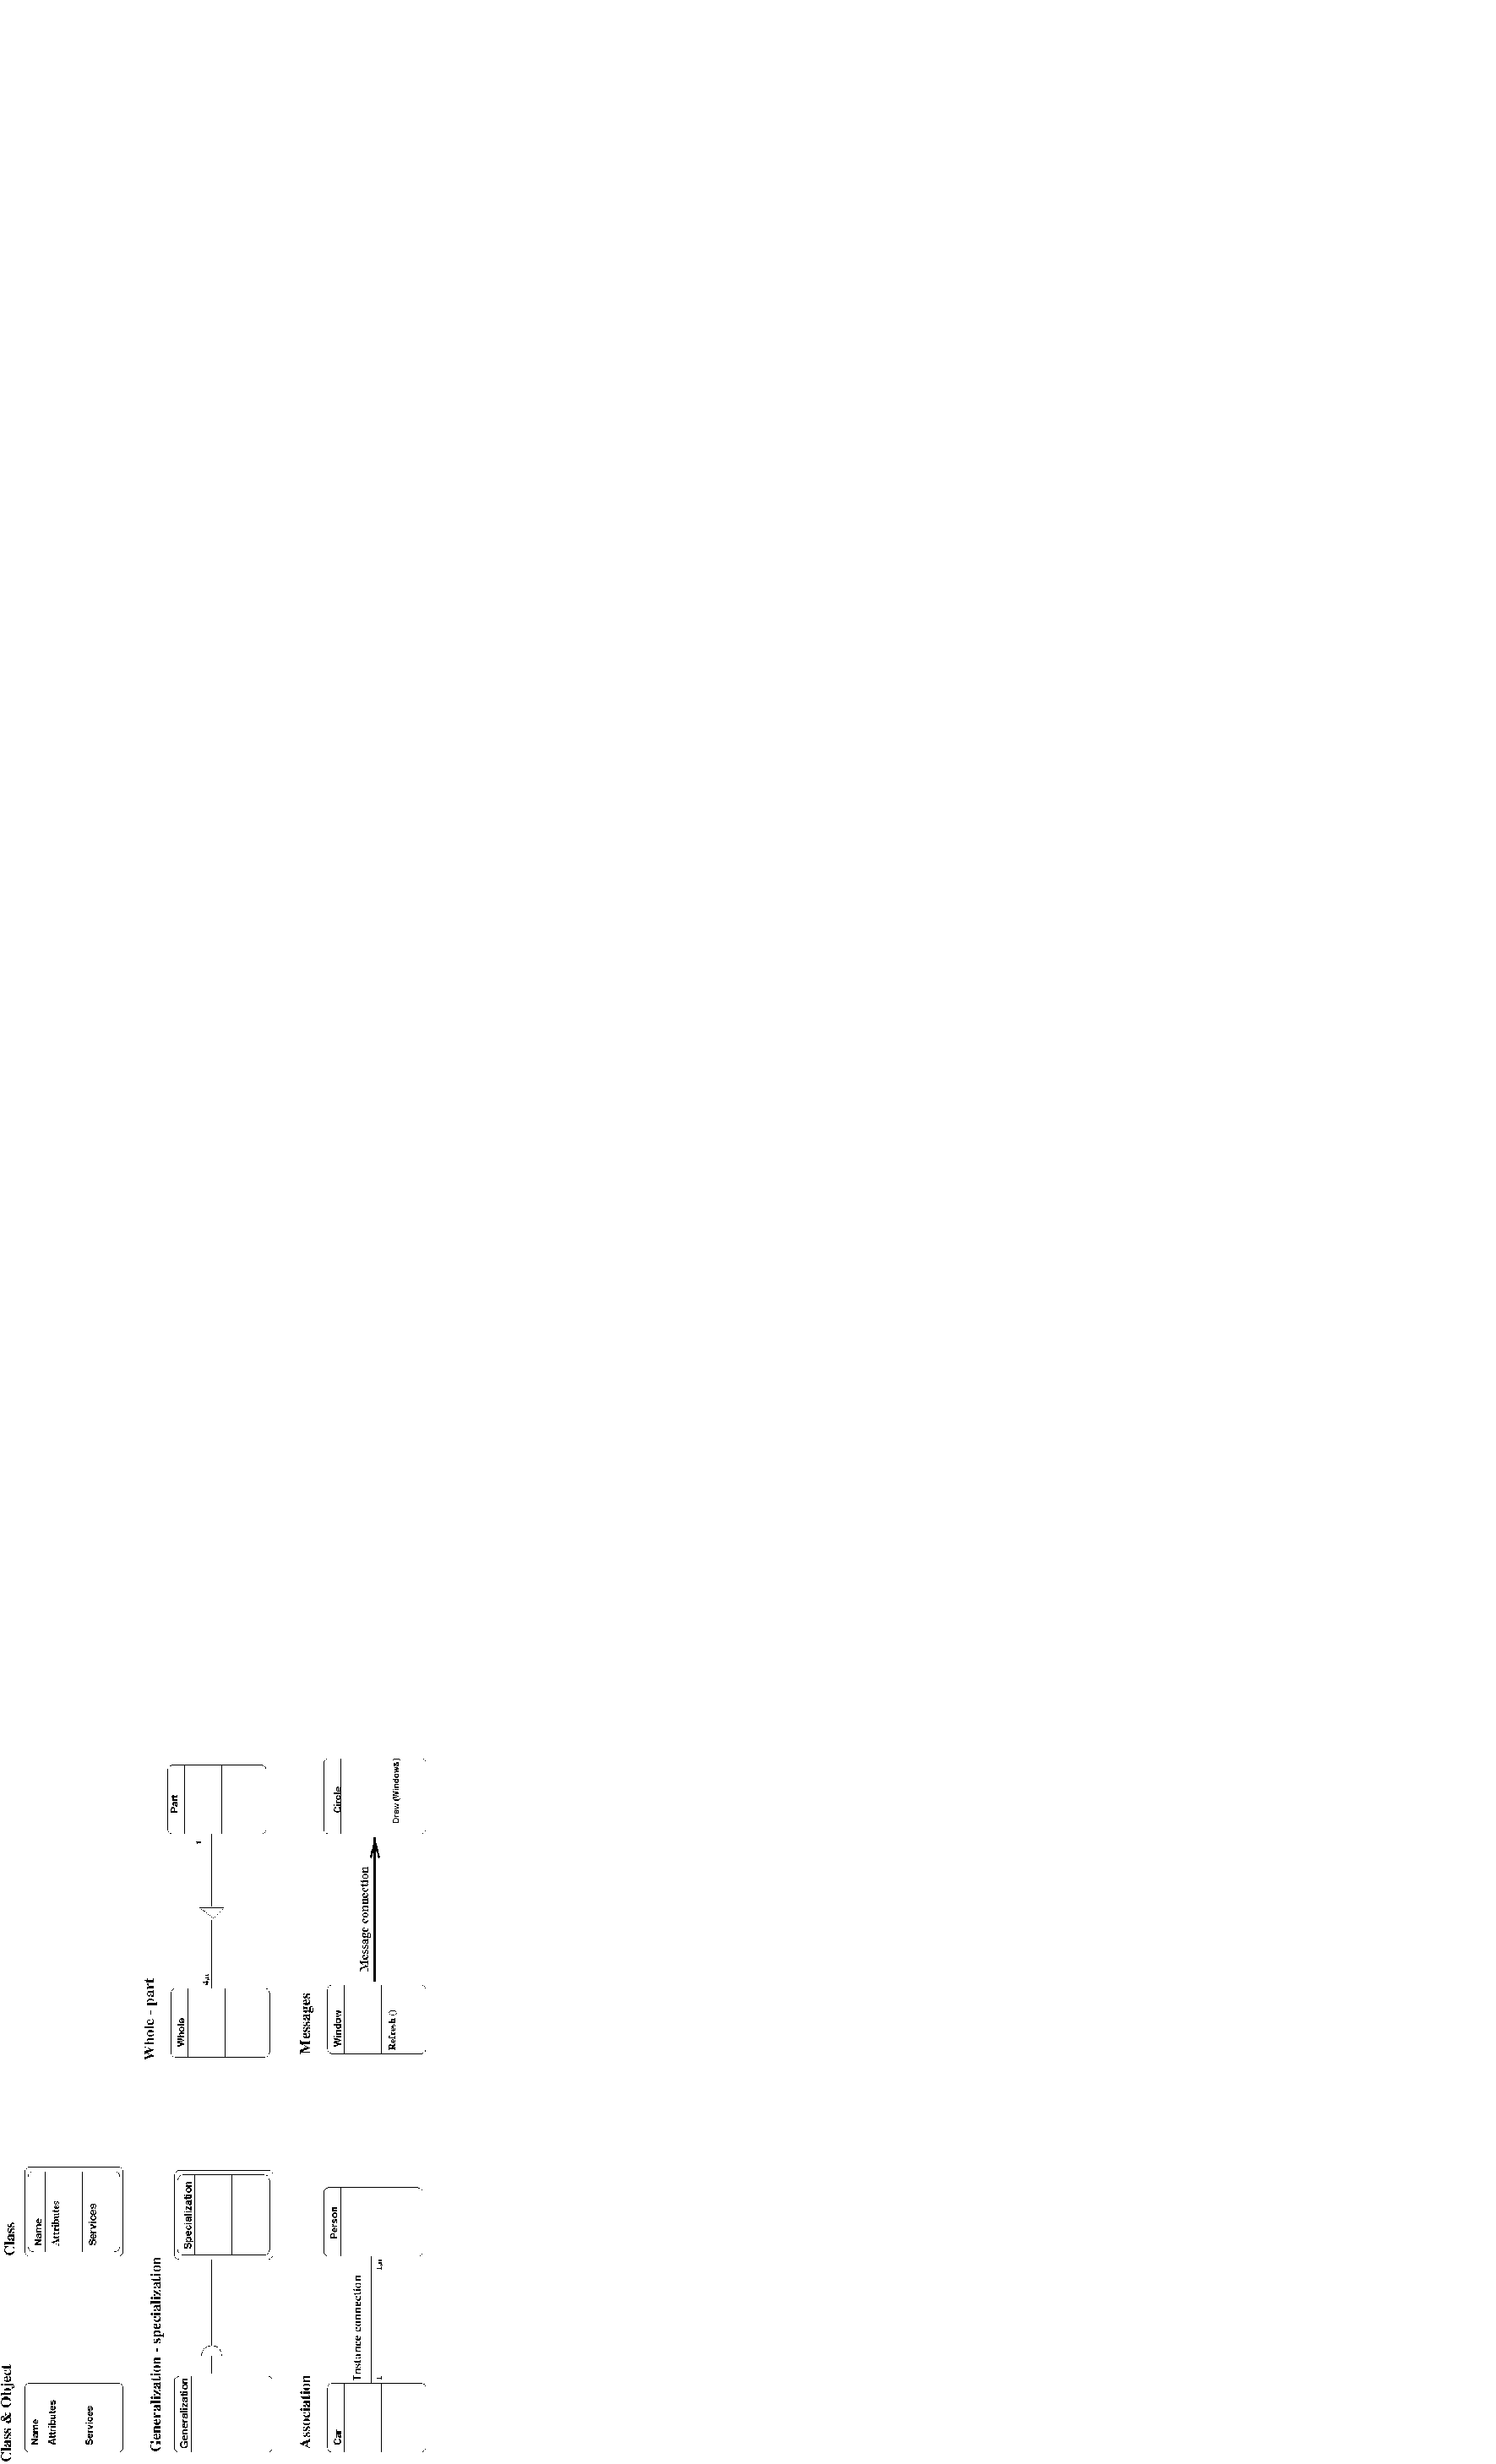
\includegraphics[width=0.7\textwidth]{coyo.pdf}}
\else
\centerline{\includegraphics[width=0.7\textwidth]{coyo.eps}}
\fi
%end{latexonly}
\caption{Coad Yourdon methodology.}
\label{coyo}
\end{figure}


\begin{figure}[tb]
\begin{htmlonly}
  \htmlimage{thumbnail=0.9,flip=r270}
  \centerline{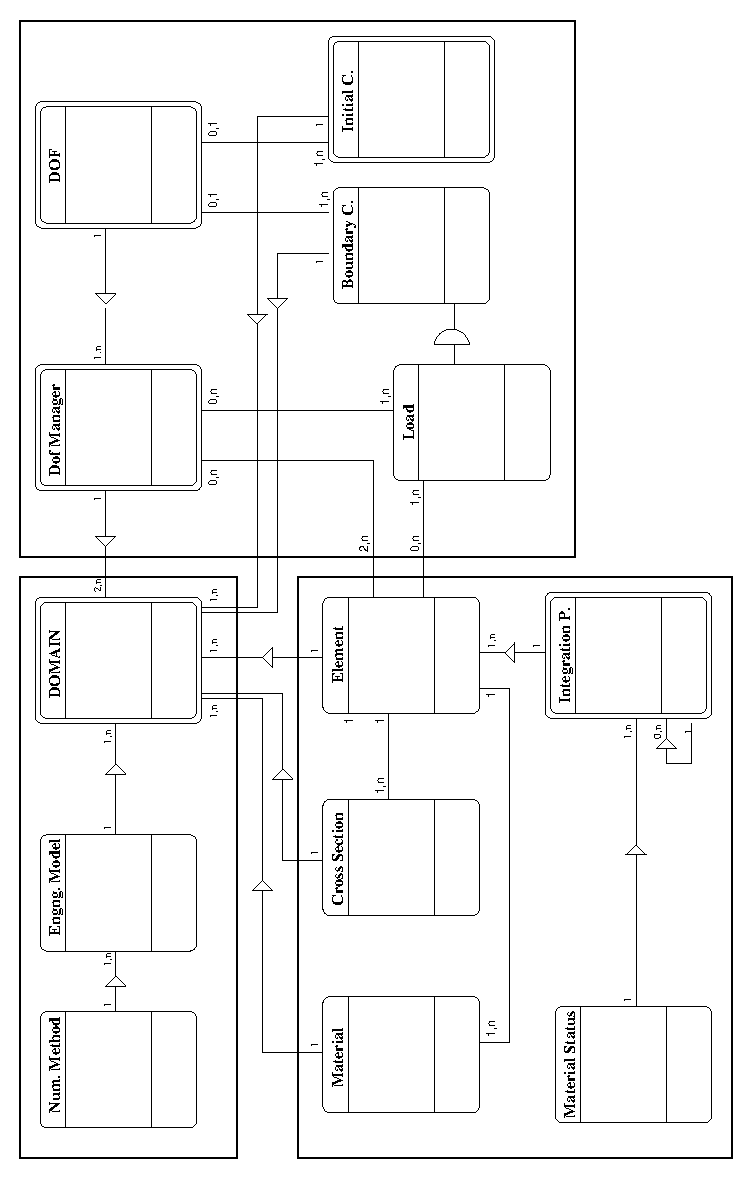
\includegraphics[width=0.7\textwidth]{general.eps}}
\end{htmlonly}
%begin{latexonly}
\ifpdf
\centerline{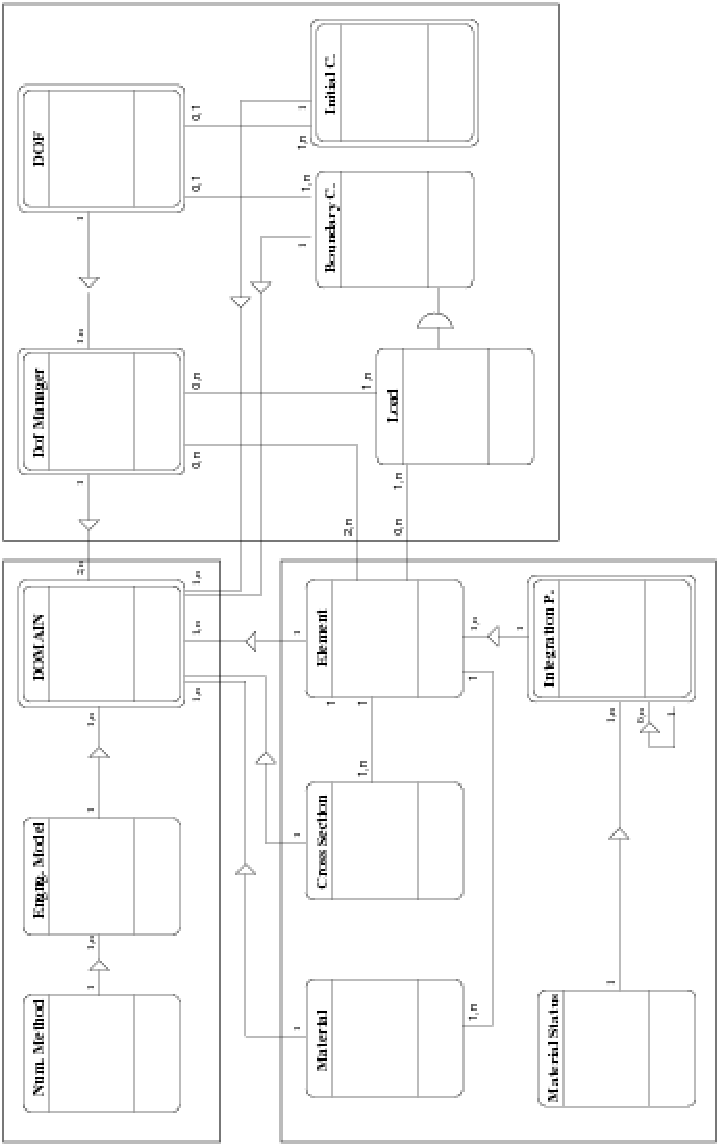
\includegraphics[width=0.7\textwidth]{general.pdf}}
\else
\centerline{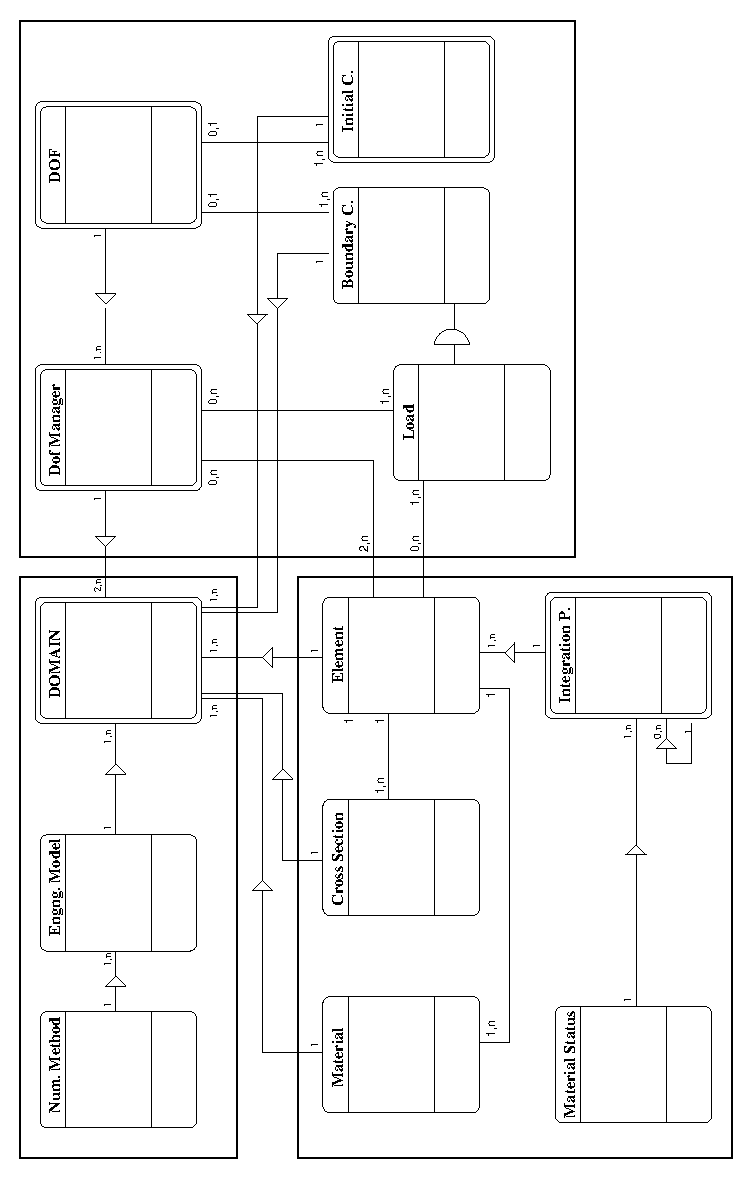
\includegraphics[width=0.7\textwidth]{general.eps}}
\fi
%end{latexonly}
\caption{General Structure.}
\label{genstructfig}
\end{figure}


\begin{figure}[tb]
\begin{htmlonly}
  \htmlimage{thumbnail=0.9,flip=r270}
  \centerline{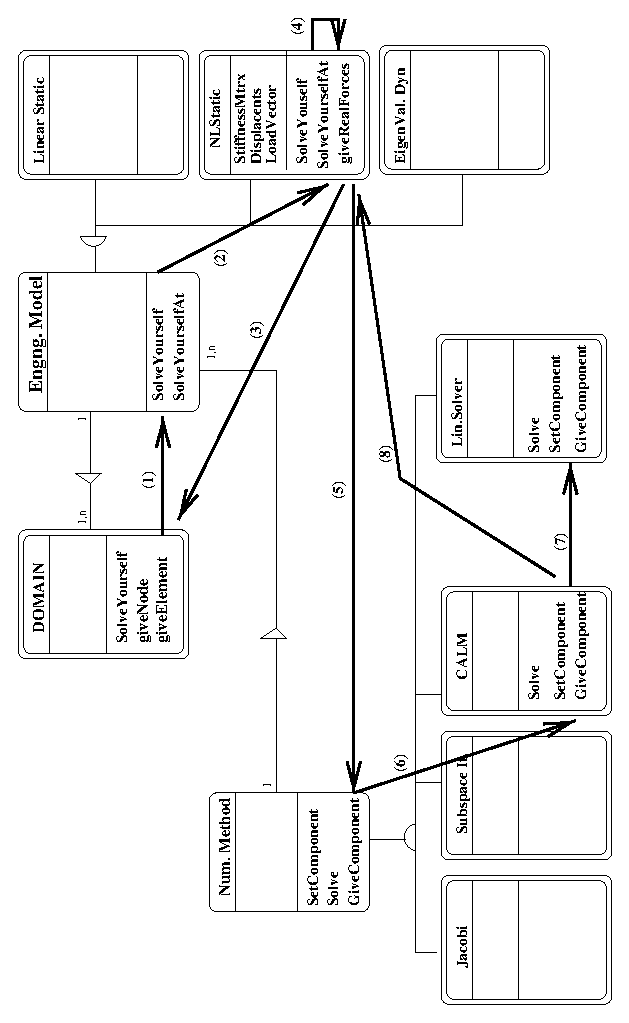
\includegraphics[width=0.7\textwidth]{struct2.eps}}
\end{htmlonly}
%begin{latexonly}
\ifpdf
\centerline{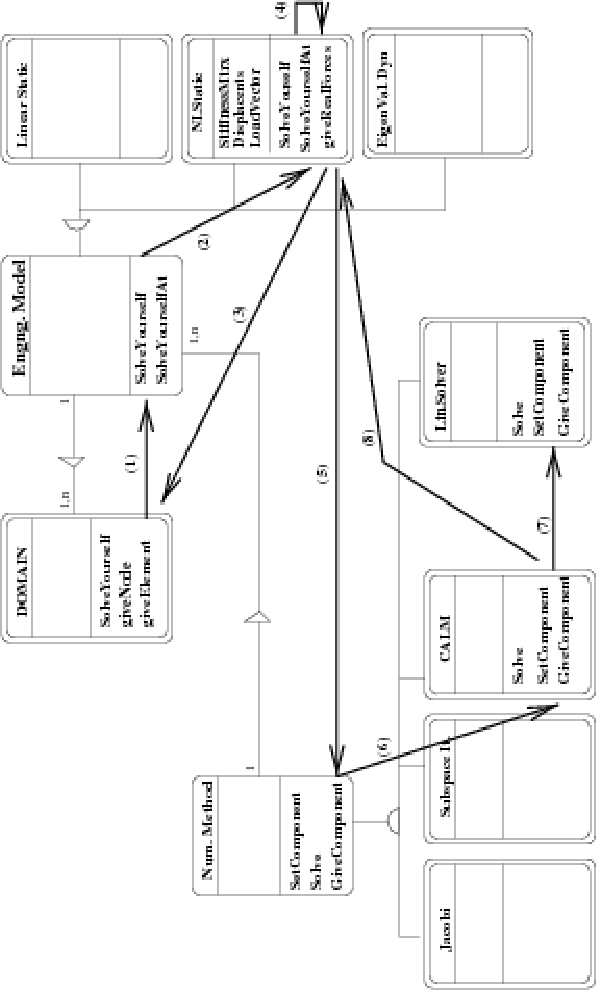
\includegraphics[width=0.7\textwidth]{struct2.pdf}}
\else
\centerline{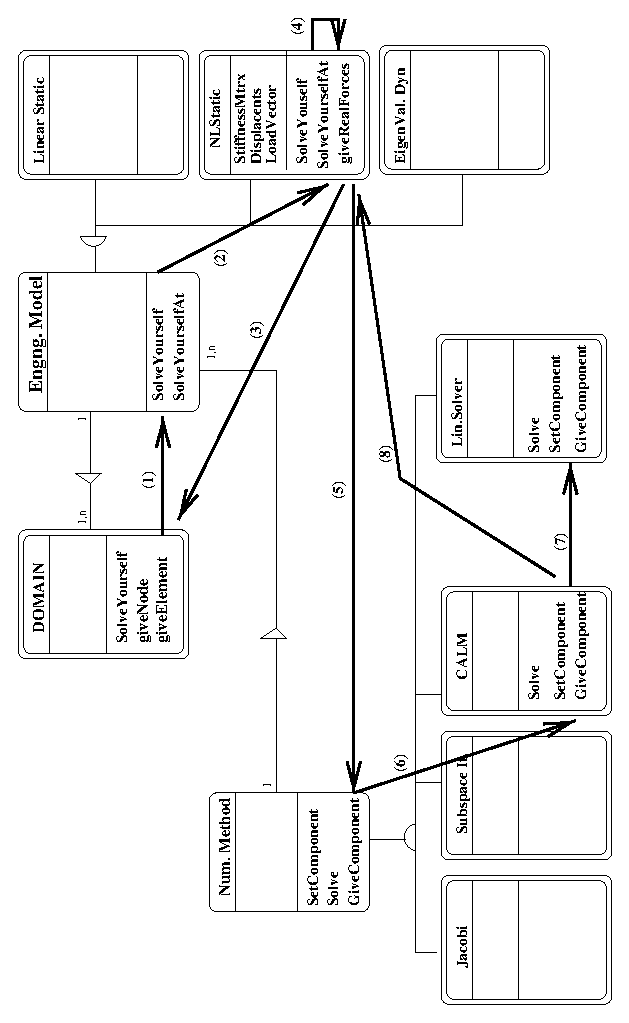
\includegraphics[width=0.7\textwidth]{struct2.eps}}
\fi
%end{latexonly}
\caption{Engng model - Numerical method Interface.}
\label{engngNummet1fig}
\end{figure}



\begin{figure}[tb]
\begin{htmlonly}
  \htmlimage{thumbnail=0.9,flip=r270}
  \centerline{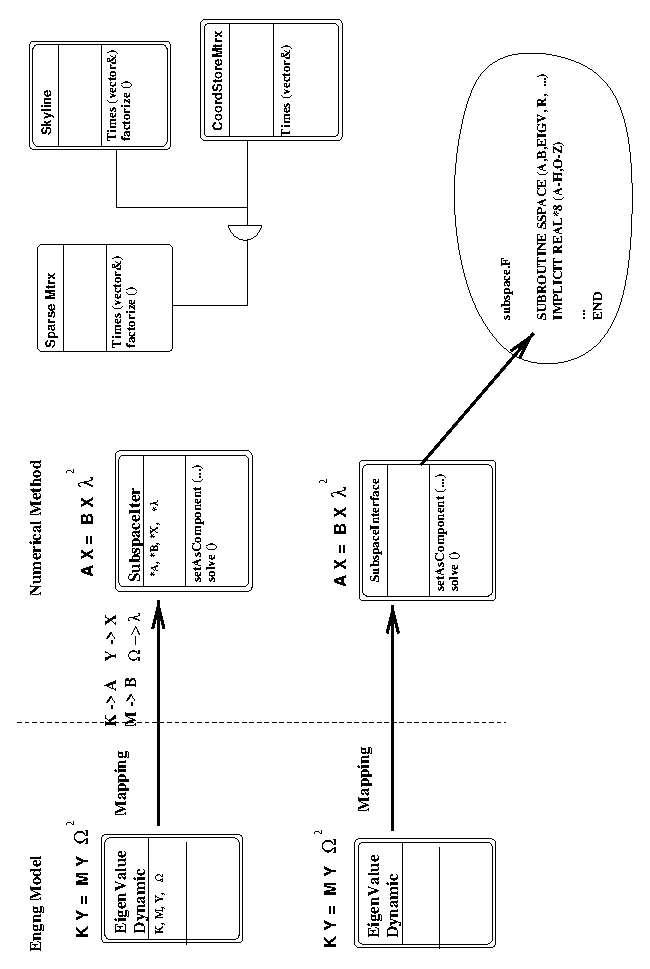
\includegraphics[width=0.7\textwidth]{engng.eps}}
\end{htmlonly}
%begin{latexonly}
\ifpdf
\centerline{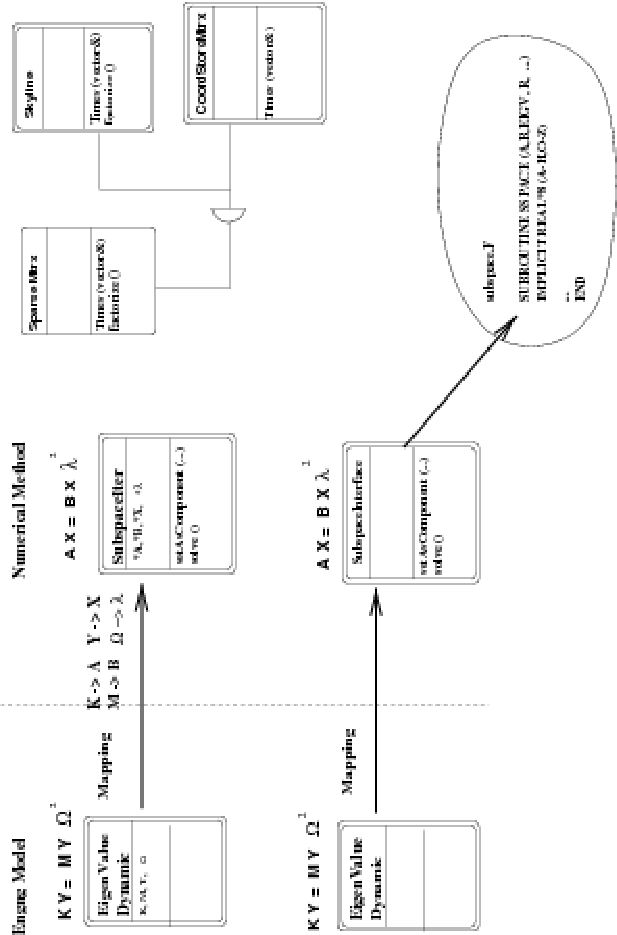
\includegraphics[width=0.7\textwidth]{engng.pdf}}
\else
\centerline{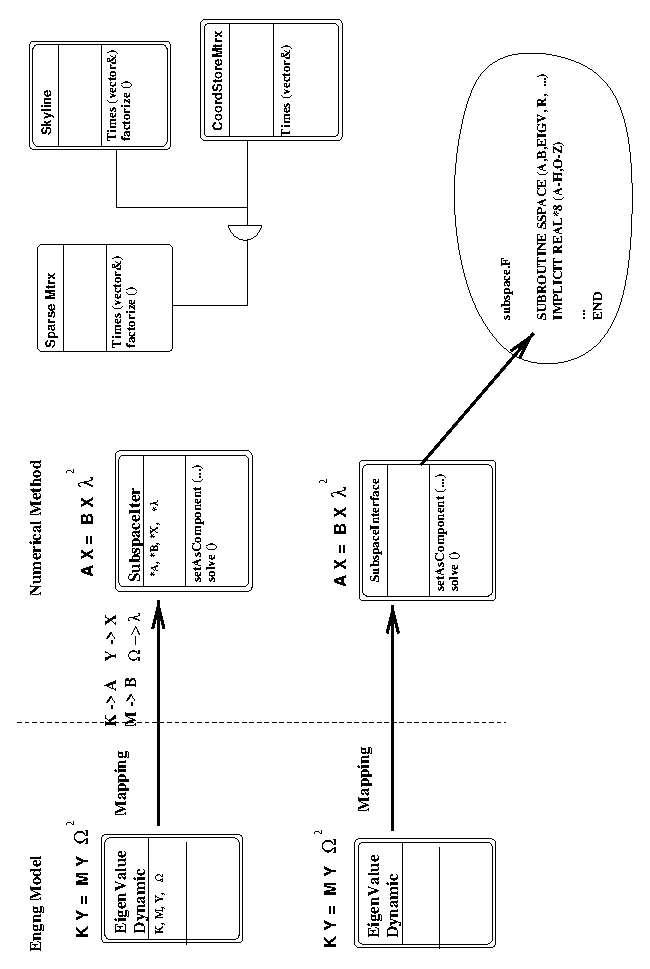
\includegraphics[width=0.7\textwidth]{engng.eps}}
\fi
%end{latexonly}
\caption{Engng model - Numerical method Interface.}
\label{engngNummet2fig}
\end{figure}



\begin{figure}[tb]
\begin{htmlonly}
  \htmlimage{thumbnail=0.9,flip=r270}
  \centerline{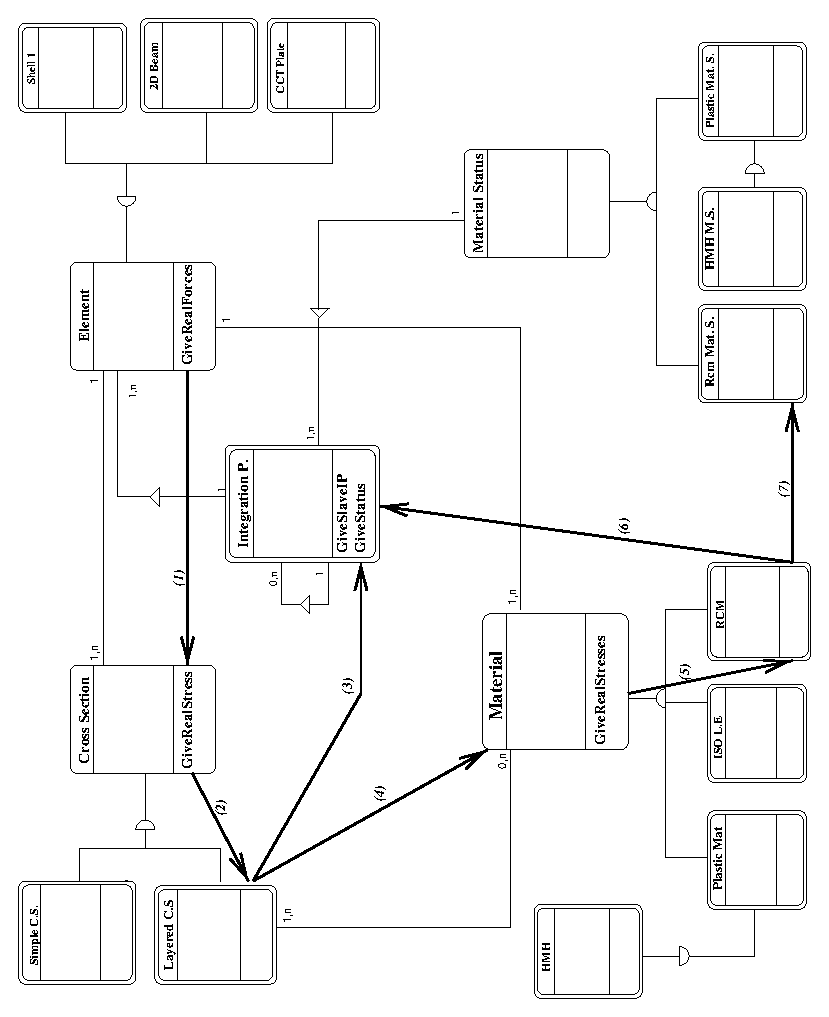
\includegraphics[width=0.7\textwidth]{struct1.eps}}
\end{htmlonly}
%begin{latexonly}
\ifpdf
\centerline{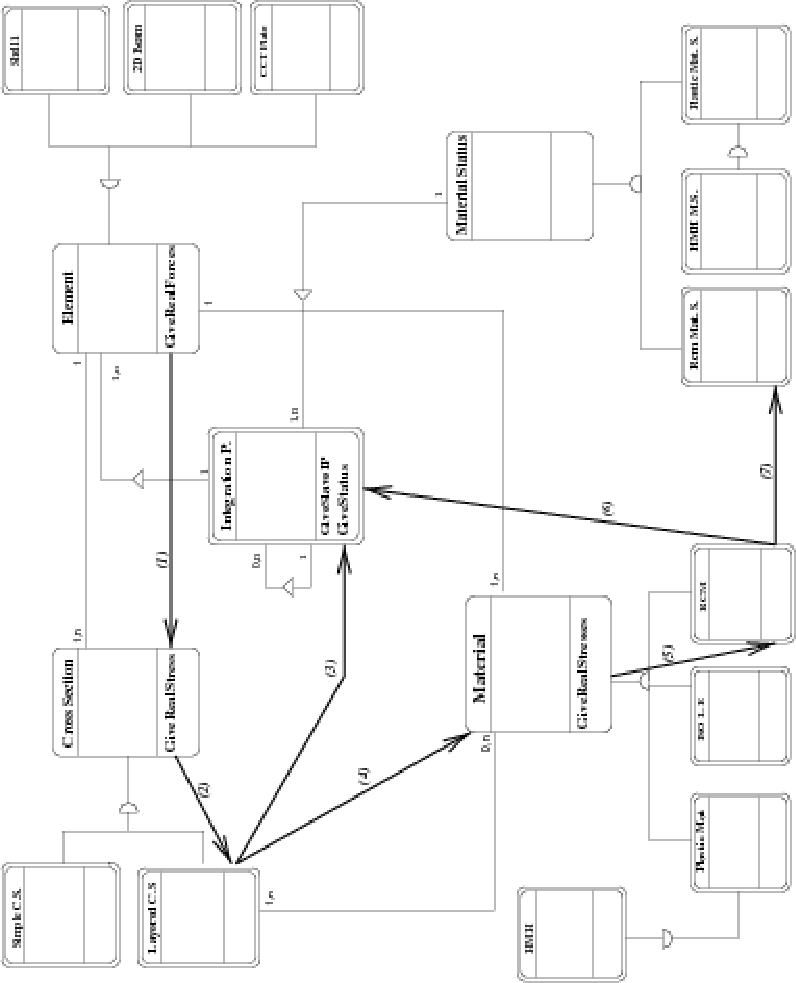
\includegraphics[width=0.7\textwidth]{struct1.pdf}}
\else
\centerline{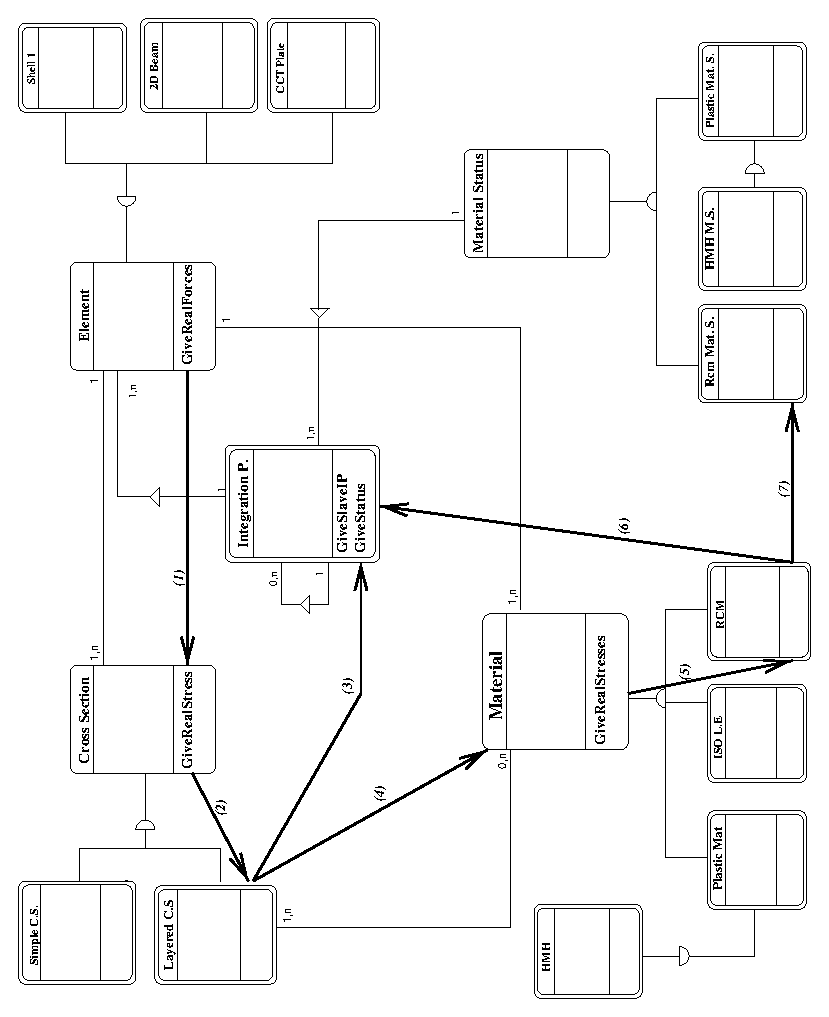
\includegraphics[width=0.7\textwidth]{struct1.eps}}
\fi
%end{latexonly}
\caption{Element-material frame  structure.}
\label{materelementFrame1}
\end{figure}

\begin{figure}[tb]
\begin{htmlonly}
  \htmlimage{thumbnail=0.9,flip=r270}
  \centerline{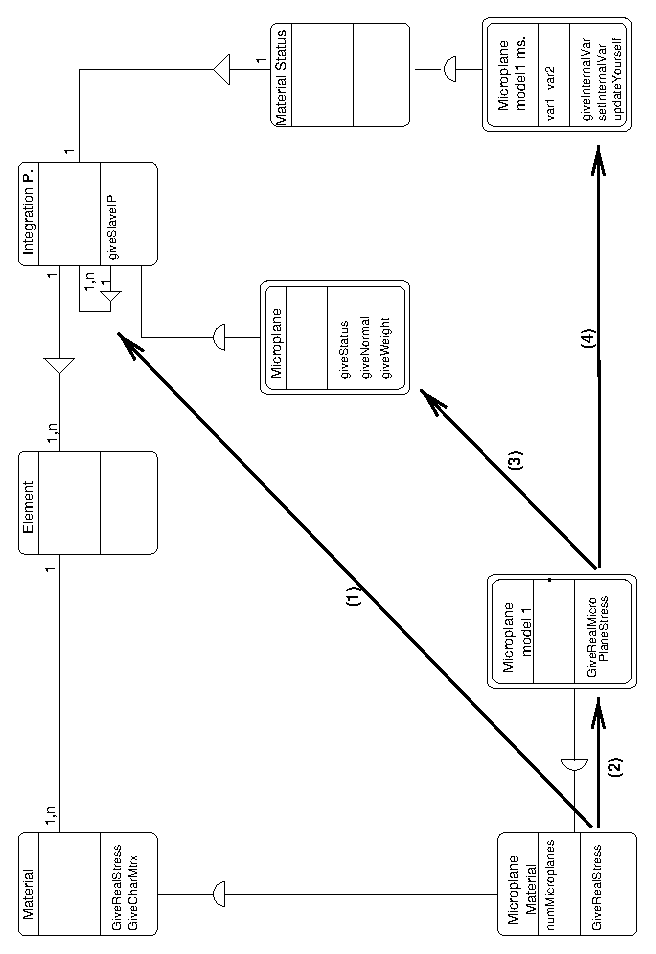
\includegraphics[width=0.7\textwidth]{microp.eps}}
\end{htmlonly}
%begin{latexonly}
\ifpdf
\centerline{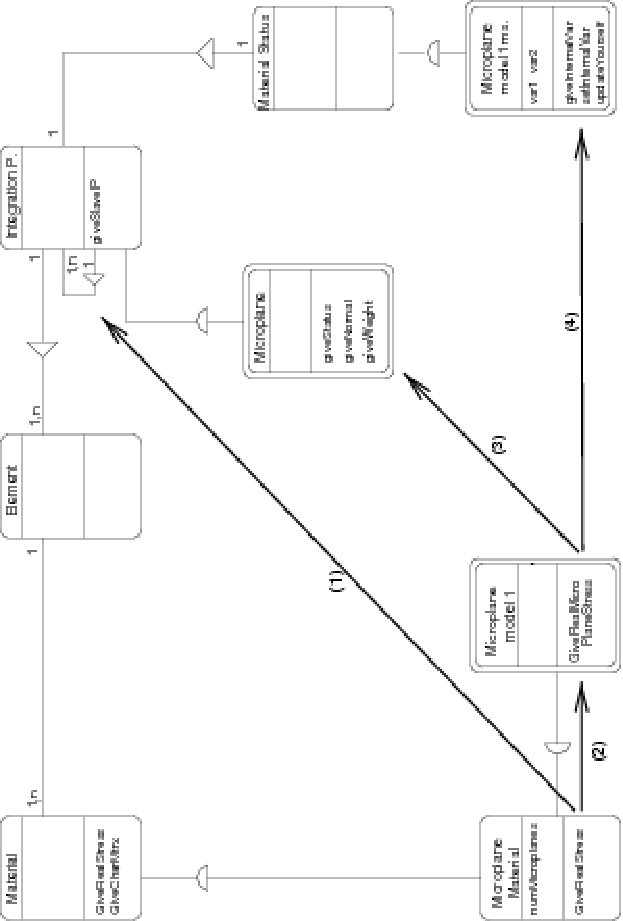
\includegraphics[width=0.7\textwidth]{microp.pdf}}
\else
\centerline{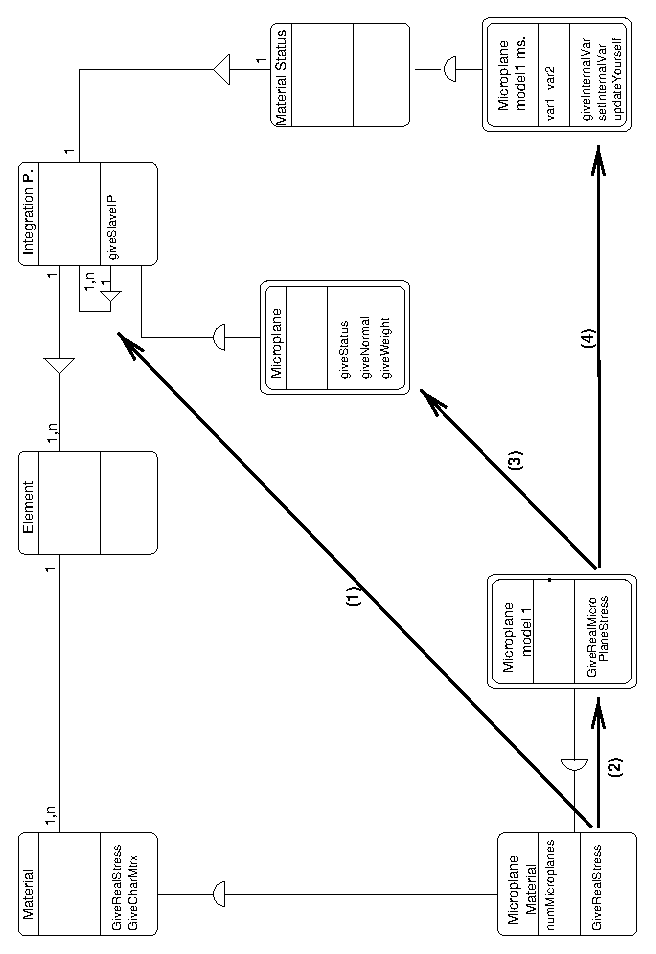
\includegraphics[width=0.7\textwidth]{microp.eps}}
\fi
%end{latexonly}
\caption{Example - Microplane model implementation.}
\label{microplaneFig}
\end{figure}



\clearpage

%\fig[t]{0mm\label{microplaneFig}\centerline{\epsfbox{microplaneSm.eps}}}           %obr.1
%{General Structure}

%\vskip20mm
%\vskip20mm
\section{Implementation}
The proposed program structure has been successfully implemented. The C++
programming language has been chosen due to its implementation
efficiency, portability, and availability. Originally, this tool has
been intended  to support material model development. Nevertheless, the
developed tool is intensively used as computational tool, thanks to
availability of implemented structural analysis module. This module
covers usual linear and non-linear static and dynamic problem
types. Large element and material libraries are provided, as well as
an interface to a mesh generator and the possibility of graphical
post-processing in X-windows. The attained computational efficiency is
comparable to existing codes. Currently, effort is devoted to parallel
processing support as well as to the development of new modules. 



\section{Conclusions}
To summarize, a general object oriented environment for finite element computations has been developed.
The described general structure leads to modular and extensible code design.
Special attention has been focused on important aspects of material library interface design, analysis type and 
numerical method representations, and corresponding interface design.
Successful implementation using C++ programming language verifies
the designed structure and provides a robust computational tool for finite
element modeling.

\section*{Acknowledgments}
This work was supported by the Grant Agency of the Czech Republic -
Project No.: 103/97/P106.

%\vfill
\begin{thebibliography}{9}

\bibitem{CoadYourdon}COAD, P. and YOURDON, E.: {Object-Oriented Analysis,} Prentice-Hall,  1991.

\bibitem{ke-ri} KERNINGHAM, B.W. and RITCHIE, D.M.: {The C Programming
Language,} Prentice-Hall, 1978.

\bibitem{pat} PATZ\'{A}K, B: {V\'{y}po\v{c}etn\'{\i} modely pro beton,} PhD
thesis, in Czech, FSv \v{C}VUT 1996. 

\bibitem{c++} STROUSTRUP, B.: {The C++ Programming Language - 3rd ed,}
Addison-Wesley, 1997.

\bibitem{zimm} ZIMMERMANN, T., DUBOIS-PELERIN, Y., and BOMME, P.: {Object-oriented finite element programming: I. Governing principles,} Comp. Meth. in Appl. Mech. Engng., 98(3), 291-303, 1992. 
\end{thebibliography}

%\newpage
%\cztitle{Objektov\v{e} orientovan\'{e} modelov\'{a}n\'{\i} metodou
%kone\v{c}n\'{y}ch prvk\accent 23u}

%\begin{resume}
%V p\v{r}\'{\i}sp\v{e}vku je prezentov\'{a}n n\'{a}vrh objektov\v{e}
%orientovan\'{e} struktury obecn\'{e}ho kone\v{c}n\v{e} prvkov\'{e}ho
%programu. Struktura je navr\v{z}ena zejm\'{e}na s ohledem na snadnou
%roz\v{s}i\v{r}itelnost a modularitu. Detailn\'{\i} pozornost je
%v\v{e}nov\'{a}na n\'{a}vrhu materialov\'{e}ho rozhran\'{\i} a
%n\'{a}vrhu rozhran\'{\i} mezi abstrakcemi reprezentuj\'{\i}c\'{\i}mi
%typ anal\'{y}zy a numerickou metodu. Navr\v{z}en\'{a} programov\'{a}
%struktura byla \'{u}sp\v{e}\v{s}n\v{e} implementov\'{a}na v C++.

%\end{resume}

%\vfill

%\received{1998}{15}{09}

%\signature{Dr. Ing. Bo\v{r}ek Patz\'{a}k.\\
%CTU, Faculty of Civil Engineering\\
%Dept. of Structural Mechanics (K132)\\
%Th\'{a}kurova 7, 166 29 Praha 6\\
%Tel.: (+420) (2) 2435 4369\\
%E-mail: bp@power4.fsv.cvut.cz}
%\makesignature
\end{document}


